% ============================================================
% RAPPORT DE MINI PROJET — Gestion des Terrains Sportifs
% Compiler : pdflatex rapport.tex (2 fois)
% ============================================================
\documentclass[12pt, a4paper]{report}

% ---- Encodage et langue ----
\usepackage[utf8]{inputenc}
\usepackage[T1]{fontenc}
\usepackage{lmodern}
\usepackage{microtype}
\usepackage[french]{babel}

% ---- Symboles spéciaux ----
\usepackage{pifont}
\newcommand{\cmark}{\ding{51}}
\newcommand{\xmark}{\ding{55}}

% ---- Mise en page ----
\usepackage[top=2.5cm, bottom=2.5cm, left=2.8cm, right=2.5cm, headheight=15pt]{geometry}
\usepackage{setspace}
\onehalfspacing
\usepackage[defaultlines=4,all]{nowidow}
\usepackage{parskip}
\setlength{\parskip}{6pt}

% ---- Graphiques et couleurs ----
\usepackage{graphicx}
\usepackage[dvipsnames]{xcolor}
\definecolor{primary}{RGB}{29, 78, 216}
\definecolor{muted}{RGB}{75, 85, 99}

% ---- Tableaux ----
\usepackage{booktabs}
\usepackage{array}
\usepackage{longtable}
\usepackage{multirow}
\usepackage{tabularx}

% ---- Style des titres ----
\usepackage{titlesec}
\titleformat{\chapter}[block]
  {\Large\bfseries\color{primary}}
  {\thechapter.\quad}{0pt}{}
  [\vspace{2pt}\color{primary}\hrule\vspace{4pt}]
\titlespacing*{\chapter}{0pt}{18pt}{14pt}

\titleformat{\section}{\large\bfseries\color{muted}}{\thesection.\quad}{0pt}{}
\titlespacing*{\section}{0pt}{12pt}{6pt}

\titleformat{\subsection}{\normalsize\bfseries}{\thesubsection.\quad}{0pt}{}
\titlespacing*{\subsection}{0pt}{10pt}{4pt}

% ---- En-têtes et pieds de page ----
\usepackage{fancyhdr}
\pagestyle{fancy}
\fancyhf{}
\fancyhead[L]{\small\itshape\color{muted}Gestion des Terrains Sportifs}
\fancyhead[R]{\small\itshape\color{muted}Rapport de Mini Projet}
\fancyfoot[C]{\small\thepage}
\renewcommand{\headrulewidth}{0.3pt}

% ---- Liens ----
\usepackage[hidelinks]{hyperref}

% ============================================================
\begin{document}

% ============================================================
%  PAGE DE GARDE
% ============================================================
\begin{titlepage}
\thispagestyle{empty}
\noindent
\includegraphics[width=3.8cm]{rapport/logo.png}
\vspace{0.8cm}
\begin{center}
{\fontsize{11}{14}\selectfont
\textbf{ÉCOLE SUPÉRIEURE PRIVÉE DES TECHNOLOGIES DE}\\
\textbf{L'INFORMATION ET DE MANAGEMENT DE NABEUL}}
\vspace{3.2cm}

{\fontsize{24}{30}\selectfont\bfseries\color{primary} Gestion des Terrains Sportifs}
\vspace{0.5cm}

{\color{primary}\rule{0.6\textwidth}{1.5pt}}
\vspace{1.2cm}

{\fontsize{12}{16}\selectfont
Présenté dans le cadre de \textbf{Mini Projet Intelligent}}
\vspace{0.4cm}

{\fontsize{12}{16}\selectfont\textbf{Spécialité :} 2\up{ème} CP A}
\vspace{1.6cm}

{\fontsize{12}{16}\selectfont\textbf{Réalisé par :}\\[0.4em]
Sarra Chorfane \quad\&\quad Mokhtar Znaidi}
\vspace{0.7cm}

{\fontsize{12}{16}\selectfont\textbf{Encadrante :} Mme Jihen Hedhli}
\vfill
{\small\color{muted} Année universitaire \textbf{2025--2026}}
\end{center}
\end{titlepage}

\tableofcontents
\newpage

% ============================================================
\chapter{Introduction}
% ============================================================

\section{Contexte du projet}

Dans le cadre du module de développement d'applications Java, nous avons réalisé
un mini projet dont le but est de créer un système de gestion des réservations
de terrains sportifs. Ce projet nous a permis de mettre en pratique plusieurs
notions importantes vues en cours : la programmation orientée objet, l'architecture
MVC, l'accès aux bases de données avec JDBC, et la création d'interfaces graphiques
avec JavaFX.

L'idée de ce projet vient d'un problème courant dans les clubs sportifs : la
gestion des réservations se fait souvent à la main (par téléphone ou sur papier),
ce qui cause des erreurs comme des créneaux réservés deux fois, des oublis ou
des erreurs dans les prix. Une application informatique permet de résoudre ces
problèmes en centralisant toutes les informations et en automatisant les calculs.

\section{Objectif de l'application}

\subsection*{Titre de l'application}

\begin{center}
{\large\bfseries\color{primary}
SportsPro — Système de Gestion des Réservations de Terrains Sportifs}
\end{center}

\subsection*{Présentation de l'application}

\textbf{SportsPro} est une application de bureau développée en Java avec une
interface graphique créée avec JavaFX 21. L'application est destinée à deux types
d'utilisateurs :

\begin{itemize}
  \item Les \textbf{clients} (les membres du club) peuvent créer un compte,
        consulter les terrains, faire des réservations, les annuler et voir
        leur historique.
  \item Les \textbf{administrateurs} peuvent gérer les terrains et les utilisateurs,
        consulter toutes les réservations, et voir des statistiques sur
        l'activité du club.
\end{itemize}

L'application assure la \textbf{sécurité} des données (les mots de passe sont
cryptés), la \textbf{fiabilité} (les conflits de créneaux sont détectés
automatiquement) et une bonne \textbf{ergonomie} (interface simple avec navigation
par onglets et plusieurs thèmes visuels).

% ============================================================
\chapter{Étude préalable}
% ============================================================

\section{Acteurs principaux}

L'application est utilisée par deux types d'acteurs qui ont des droits différents :

\begin{center}
\begin{tabular}{>{\bfseries}p{3.8cm} p{9.2cm}}
\toprule
Acteur & Description \\
\midrule
Administrateur &
  C'est le gestionnaire du club. Il a accès à toutes les fonctionnalités :
  gérer les terrains, voir et annuler toutes les réservations, gérer les
  comptes des utilisateurs et consulter les statistiques. \\
\addlinespace
Client &
  C'est un membre du club. Il peut s'inscrire, se connecter, réserver un
  terrain, annuler ses réservations, voir son historique et modifier
  son profil. \\
\bottomrule
\end{tabular}
\end{center}

\section{Besoins fonctionnels par acteur}

\subsection{Client}

\begin{enumerate}
  \item \textbf{Inscription et connexion} : le client peut créer un compte
        avec son nom, son e-mail et un mot de passe, puis se connecter.
  \item \textbf{Consulter les terrains} : voir la liste des terrains avec
        leur type, leur prix à l'heure et leur description.
  \item \textbf{Réserver un terrain} : choisir un terrain disponible, une
        date, une heure de début et une durée (1 à 4 heures). Le montant
        total est calculé et affiché en temps réel.
  \item \textbf{Consulter l'historique} : voir toutes ses réservations avec
        la possibilité de les filtrer par statut ou par période.
  \item \textbf{Annuler une réservation} : annuler une réservation confirmée
        si la date n'est pas encore passée.
  \item \textbf{Modifier son profil} : changer son nom, son e-mail ou son
        mot de passe.
  \item \textbf{Exporter en CSV} : télécharger la liste de ses réservations
        dans un fichier tableur.
\end{enumerate}

\subsection{Administrateur}

\begin{enumerate}
  \item \textbf{Tableau de bord} : voir quatre indicateurs importants
        (terrains utilisés, nombre de réservations, réservations confirmées,
        chiffre d'affaires) ainsi que des graphiques de répartition.
  \item \textbf{Gérer les terrains} : ajouter un nouveau terrain, l'activer
        ou le désactiver, et le supprimer.
  \item \textbf{Gérer les réservations} : voir toutes les réservations
        de tous les clients, les filtrer, les annuler et exporter en CSV.
  \item \textbf{Gérer les utilisateurs} : voir les comptes et supprimer
        un compte client.
  \item \textbf{Paramètres} : choisir le thème de l'interface, configurer
        le rafraîchissement automatique et changer le mot de passe.
\end{enumerate}

\section{Besoins non fonctionnels}

\begin{center}
\begin{tabular}{>{\bfseries}p{3.5cm} p{9.5cm}}
\toprule
Critère & Description \\
\midrule
Sécurité &
  Les mots de passe ne sont jamais stockés en clair : ils sont hachés
  avec l'algorithme BCrypt (10 rounds). Les requêtes SQL utilisent des
  \texttt{PreparedStatement} pour éviter les injections SQL. \\
\addlinespace
Performance &
  La connexion à la base de données utilise le patron Singleton pour
  éviter d'ouvrir plusieurs connexions inutiles. Les réponses sont
  affichées en moins d'une seconde. \\
\addlinespace
Fiabilité &
  Avant chaque réservation, le système vérifie automatiquement qu'il
  n'y a pas de conflit avec un créneau déjà réservé sur le même terrain. \\
\addlinespace
Maintenabilité &
  Le code est organisé en couches séparées (DAO, Service, Contrôleur,
  Vue) avec des interfaces Java. Chaque couche s'occupe d'une seule
  responsabilité. \\
\addlinespace
Portabilité &
  L'application est développée en Java, donc elle fonctionne sur
  Windows, Mac et Linux. Elle est livrée sous forme de fichier JAR
  exécutable créé avec Maven. \\
\addlinespace
Ergonomie &
  L'interface propose trois thèmes visuels (Ocean Pro, Emerald Field,
  Sunset Arena), une navigation simple par onglets et des couleurs
  différentes selon le statut des réservations. \\
\bottomrule
\end{tabular}
\end{center}

\section{Technologies utilisées}

\begin{center}
\begin{tabular}{>{\bfseries}p{3.5cm} p{2.5cm} p{7cm}}
\toprule
Technologie & Version & Utilisation \\
\midrule
Java             & 25         & Langage principal du projet \\
JavaFX           & 21.0.5     & Création de l'interface graphique \\
MySQL            & 8.0        & Base de données relationnelle \\
JDBC             & JDK natif  & Connexion entre Java et MySQL \\
jBCrypt          & 0.4        & Hachage des mots de passe \\
Apache Maven     & 3.9+       & Gestion des dépendances et création du JAR \\
JUnit 5          & 5.10.1     & Tests unitaires automatisés \\
Mockito          & 5.17.0     & Simulation des dépendances dans les tests \\
\bottomrule
\end{tabular}
\end{center}

% ============================================================
\chapter{Conception}
% ============================================================

\section{Diagramme de cas d'utilisation globale}

Le diagramme ci-dessous montre toutes les fonctionnalités de l'application et
les acteurs qui peuvent les utiliser. Le \textbf{Client} a accès aux opérations
liées à ses réservations, et l'\textbf{Administrateur} a accès à la gestion
complète du système.

\begin{figure}[htbp]
\centering
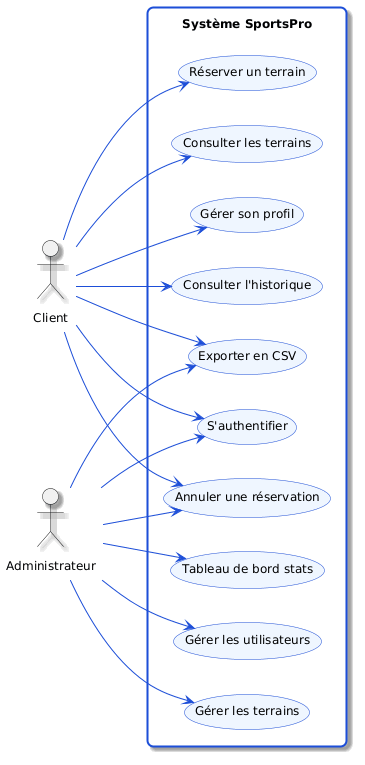
\includegraphics[width=0.95\textwidth,height=0.78\textheight,keepaspectratio]{rapport/images/01_diagramme-cas_utilisation.png}
\caption{Diagramme de cas d'utilisation global — SportsPro}
\label{fig:usecase}
\end{figure}

\section{Description textuelle d'un cas d'utilisation essentielle}

Parmi tous les cas d'utilisation, nous avons choisi de décrire en détail
la réservation d'un terrain car c'est la fonctionnalité centrale de
l'application.

\vspace{0.4cm}
\begin{center}
\begin{tabular}{>{\bfseries}p{4.2cm} p{8.8cm}}
\toprule
Nom & Réserver un terrain \\
\midrule
Acteur principal & Client \\
\addlinespace
Préconditions &
  Le client est connecté à l'application.
  Au moins un terrain est disponible. \\
\addlinespace
Postconditions &
  La réservation est enregistrée avec le statut \texttt{CONFIRMEE}.
  Le montant est calculé automatiquement (prix/h $\times$ durée). \\
\addlinespace
Scénario principal &
  \begin{enumerate}
    \item Le client ouvre l'onglet \textit{Nouvelle Réservation}.
    \item Il choisit un terrain dans la liste des terrains disponibles.
    \item Il sélectionne une date, une heure de début et une durée.
    \item Le montant estimé s'affiche et se met à jour en direct.
    \item Il clique sur \textit{Confirmer la réservation}.
    \item Le système vérifie qu'il n'y a pas de conflit de créneau.
    \item La réservation est enregistrée et une confirmation s'affiche.
  \end{enumerate} \\
\addlinespace
Cas alternatifs &
  \textbf{6a.} Un conflit est détecté : un message d'erreur s'affiche
  et la réservation est refusée. \\
& \textbf{3a.} La date choisie est dans le passé : le champ est bloqué. \\
\addlinespace
Règles métier &
  Les réservations sont possibles de 08h00 à 22h00, pour une durée
  de 1 à 4 heures. Deux créneaux $[A,B]$ et $[C,D]$ se chevauchent
  si $A < D$ \textbf{et} $C < B$. \\
\bottomrule
\end{tabular}
\end{center}

\section{Diagramme de classe}

Le diagramme de classes montre les trois entités principales de l'application
(\texttt{Utilisateur}, \texttt{Terrain}, \texttt{Reservation}) et les trois
énumérations (\texttt{Role}, \texttt{TypeTerrain}, \texttt{StatutReservation})
avec leurs attributs et leurs relations.

\begin{figure}[htbp]
\centering
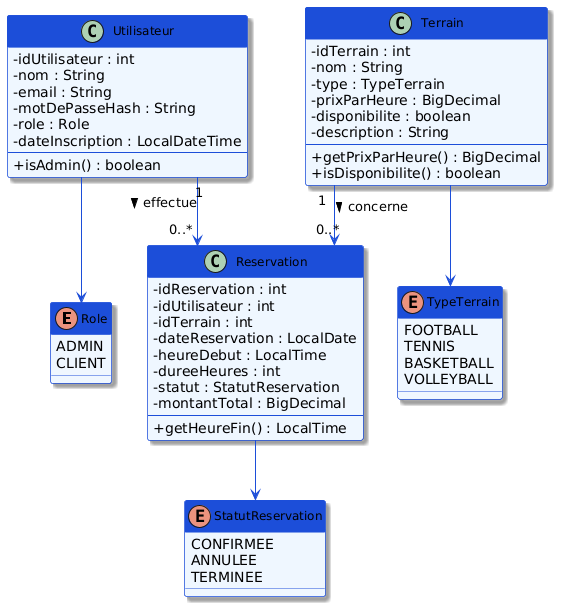
\includegraphics[width=0.95\textwidth]{rapport/images/02_diagramme_classes.png}
\caption{Diagramme de classes — projet SportsPro}
\label{fig:classes}
\end{figure}

\section{Diagramme de séquence}

Ce diagramme montre le déroulement complet de la réservation d'un terrain,
depuis le moment où le client clique sur le bouton jusqu'à l'enregistrement
en base de données. Il présente deux cas : la réservation réussie et le
refus en cas de conflit de créneau.

\begin{figure}[htbp]
\centering
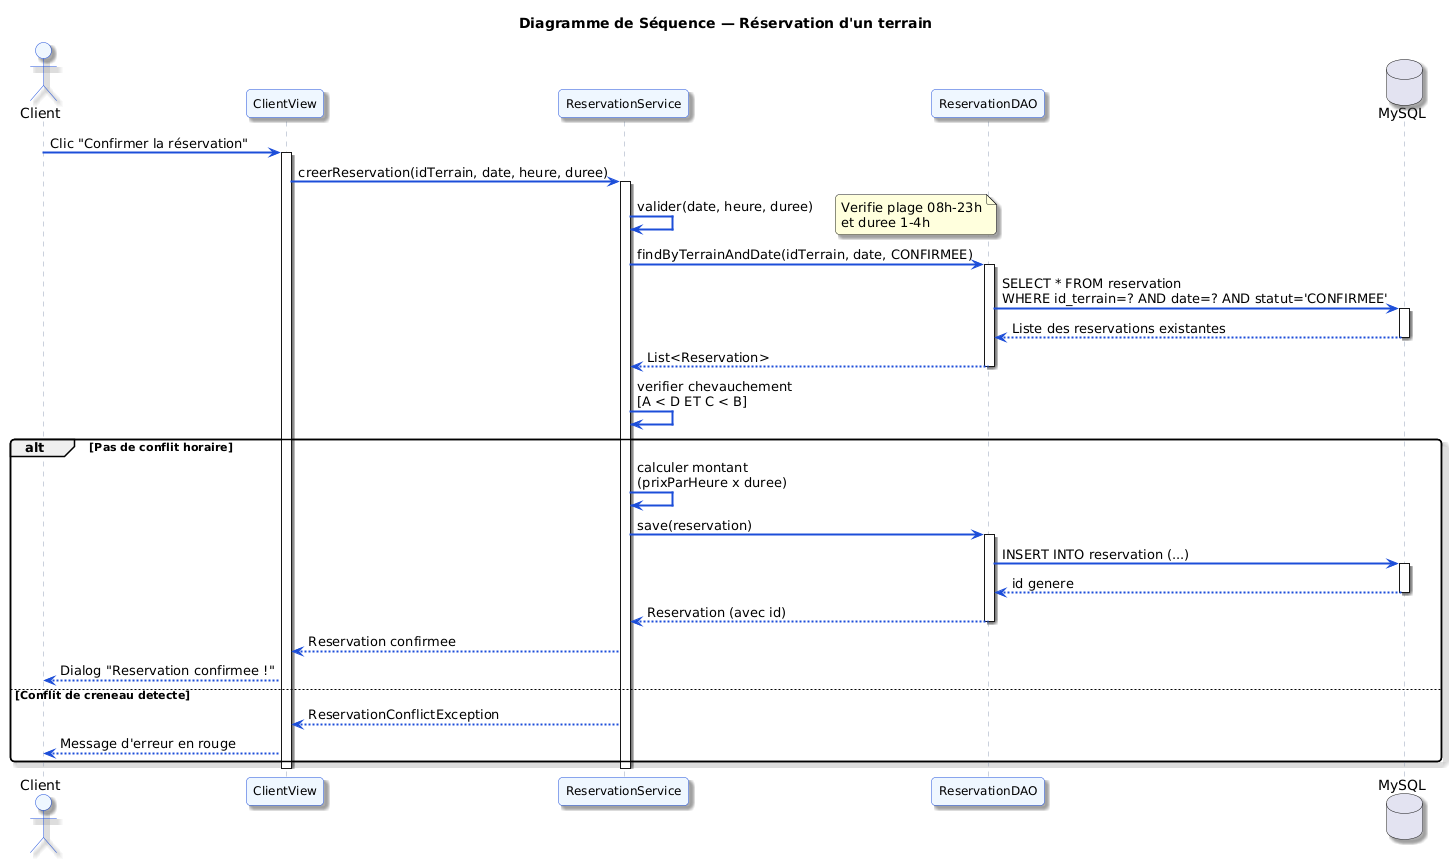
\includegraphics[width=0.95\textwidth]{rapport/images/03_diagramme_sequence.png}
\caption{Diagramme de séquence — Réservation d'un terrain}
\label{fig:sequence}
\end{figure}

% ============================================================
\chapter{Architecture}
% ============================================================

\section{Organisation du projet selon le modèle MVC}

Notre projet utilise une \textbf{architecture en couches} basée sur le modèle
\textbf{MVC} (Modèle - Vue - Contrôleur). Nous avons ajouté deux couches
supplémentaires : la couche \textbf{Service} pour la logique métier et la
couche \textbf{DAO} pour l'accès à la base de données. Chaque couche ne
communique qu'avec la couche juste en dessous, ce qui rend le code plus
organisé et plus facile à modifier.

\begin{figure}[htbp]
\centering
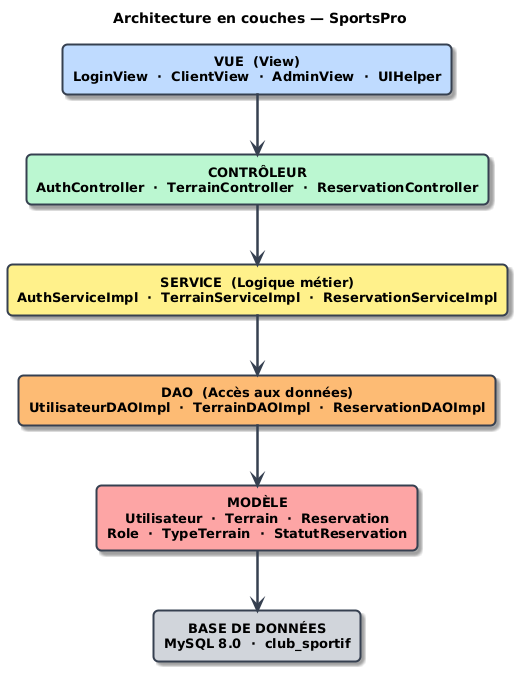
\includegraphics[width=0.82\textwidth]{rapport/images/05_architecture_mvc.png}
\caption{Architecture en couches MVC — SportsPro}
\label{fig:mvc}
\end{figure}

\begin{center}
\begin{tabular}{>{\bfseries}p{3cm} p{10cm}}
\toprule
Couche & Rôle \\
\midrule
Vue (View) &
  Les interfaces JavaFX : \texttt{LoginView}, \texttt{ClientView},
  \texttt{AdminView}, \texttt{UIHelper}. C'est ce que l'utilisateur
  voit et avec quoi il interagit. \\
\addlinespace
Contrôleur &
  \texttt{AuthController}, \texttt{TerrainController},
  \texttt{ReservationController}. Il reçoit les actions de l'utilisateur
  et appelle les bons services. \\
\addlinespace
Service &
  Contient la logique métier : vérification des données, calcul du
  montant, détection des conflits de créneaux. Implémente les interfaces
  \texttt{IAuthService}, \texttt{ITerrainService}, \texttt{IReservationService}. \\
\addlinespace
DAO &
  Fait les requêtes SQL vers la base de données via JDBC.
  Une classe par table. \\
\addlinespace
Modèle &
  Les objets Java qui représentent les données : \texttt{Utilisateur},
  \texttt{Terrain}, \texttt{Reservation} et les énumérations. \\
\addlinespace
Base de données &
  MySQL 8.0 — base \texttt{club\_sportif}, 3 tables. \\
\bottomrule
\end{tabular}
\end{center}

\section{Hiérarchie des packages}

Le projet est organisé en packages Java qui correspondent chacun à une couche
de l'architecture. Les captures suivantes, prises depuis notre environnement
de développement, montrent la structure réelle du projet avec toutes les classes
que nous avons créées.

\begin{figure}[htbp]
\centering
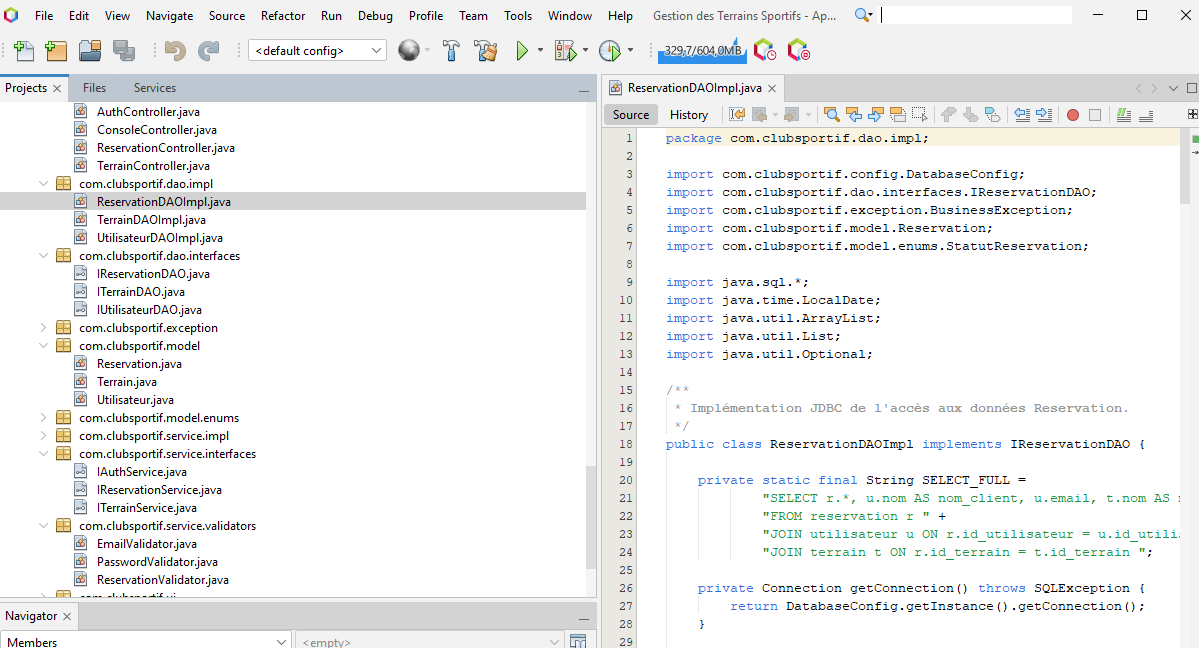
\includegraphics[width=0.82\textwidth,keepaspectratio]{rapport/images/hierachie_packages1.PNG}
\caption{Hiérarchie des packages — vue générale du projet}
\label{fig:packages1}
\end{figure}

\begin{figure}[htbp]
\centering
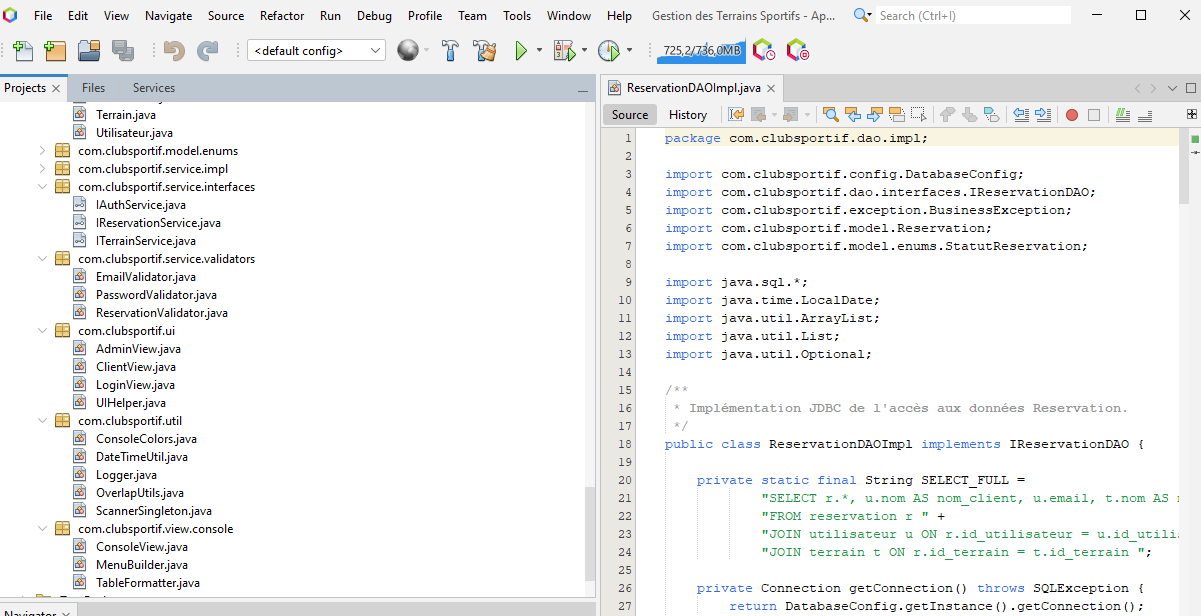
\includegraphics[width=0.82\textwidth,keepaspectratio]{rapport/images/hierachie_packages2.PNG}
\caption{Hiérarchie des packages — détail des sous-packages}
\label{fig:packages2}
\end{figure}

% ============================================================
\chapter{Réalisation}
% ============================================================

\section{Description des interfaces graphiques réalisées}

Nous avons conçu l'interface de SportsPro pour qu'elle soit simple et agréable
à utiliser. Chaque vue est adaptée au type d'utilisateur connecté : l'espace
client est axé sur la réservation, et le tableau de bord de l'administrateur
est axé sur la gestion et le suivi.

\subsection{Écran de connexion et d'inscription}

L'écran de démarrage de l'application est divisé en deux parties : le panneau
gauche présente le nom de l'application et ses fonctionnalités principales,
et le panneau droit contient le formulaire. Deux onglets permettent de passer
de l'\textbf{onglet Connexion} à l'\textbf{onglet Inscription} sans quitter
l'écran.

L'interface effectue plusieurs validations directement pendant la saisie :
\begin{itemize}
  \item Le format de l'adresse e-mail est vérifié en temps réel.
  \item Le mot de passe doit contenir au moins 8 caractères, une majuscule
        et un chiffre.
  \item Les messages d'erreur s'affichent en rouge sous chaque champ concerné.
  \item Un bouton permet de voir ou de masquer le mot de passe.
\end{itemize}

\begin{figure}[htbp]
\centering
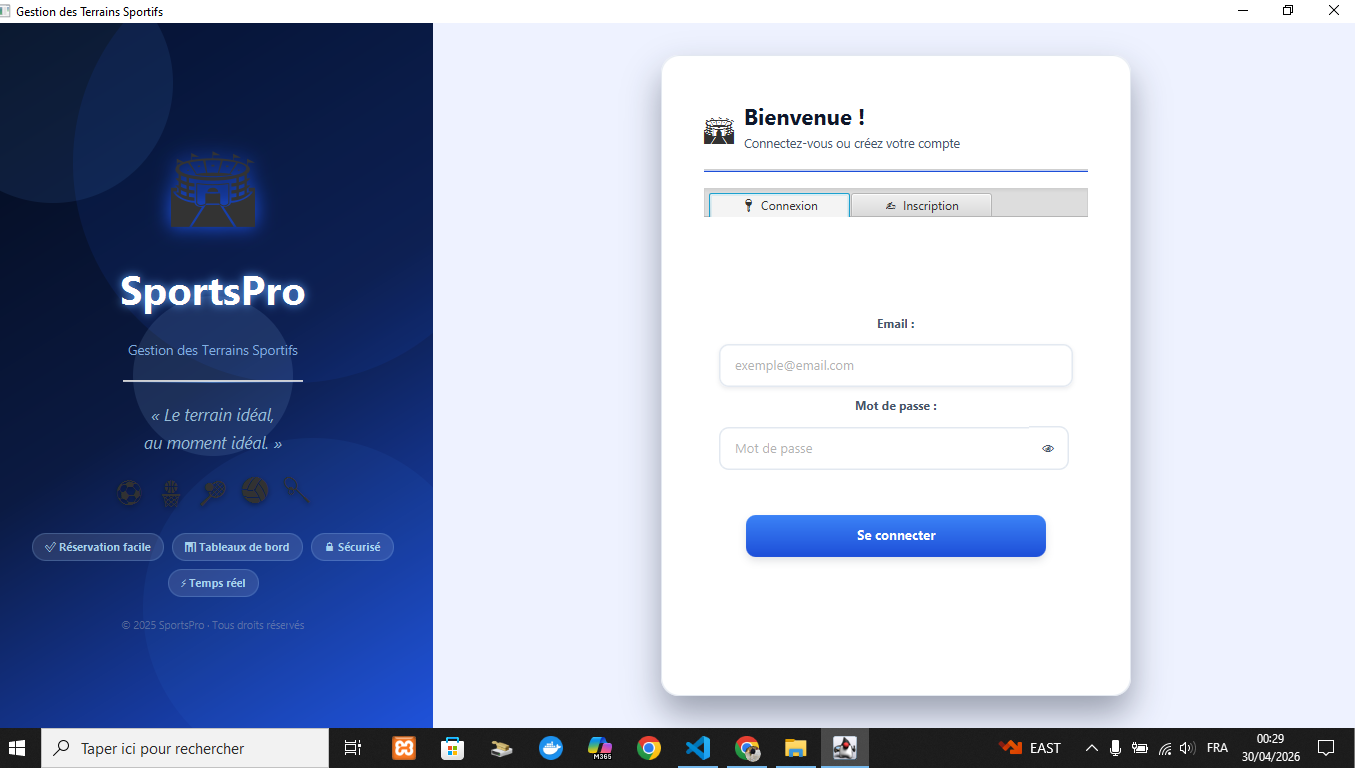
\includegraphics[width=0.92\textwidth]{rapport/images/login.PNG}
\caption{Écran de connexion et d'inscription — SportsPro}
\label{fig:login}
\end{figure}

\subsection{Tableau de bord Administrateur}

Après connexion, l'administrateur voit son tableau de bord organisé en
\textbf{cinq onglets}. En haut de l'écran, une barre de navigation affiche
son nom, son rôle (badge ADMIN) et un bouton de déconnexion.

\subsubsection*{Onglet Statistiques}

Cet onglet est le tableau de bord principal. Il affiche quatre
\textbf{indicateurs clés} (cartes KPI) : le nombre de terrains utilisés,
le nombre total de réservations, le nombre de réservations confirmées, et
le chiffre d'affaires total. Deux graphiques complètent ces informations :
un \textbf{graphique en barres} qui montre les réservations par type de terrain,
et un \textbf{graphique en secteurs} qui montre la répartition par statut
(Confirmées, Annulées, Terminées).

\begin{figure}[htbp]
\centering
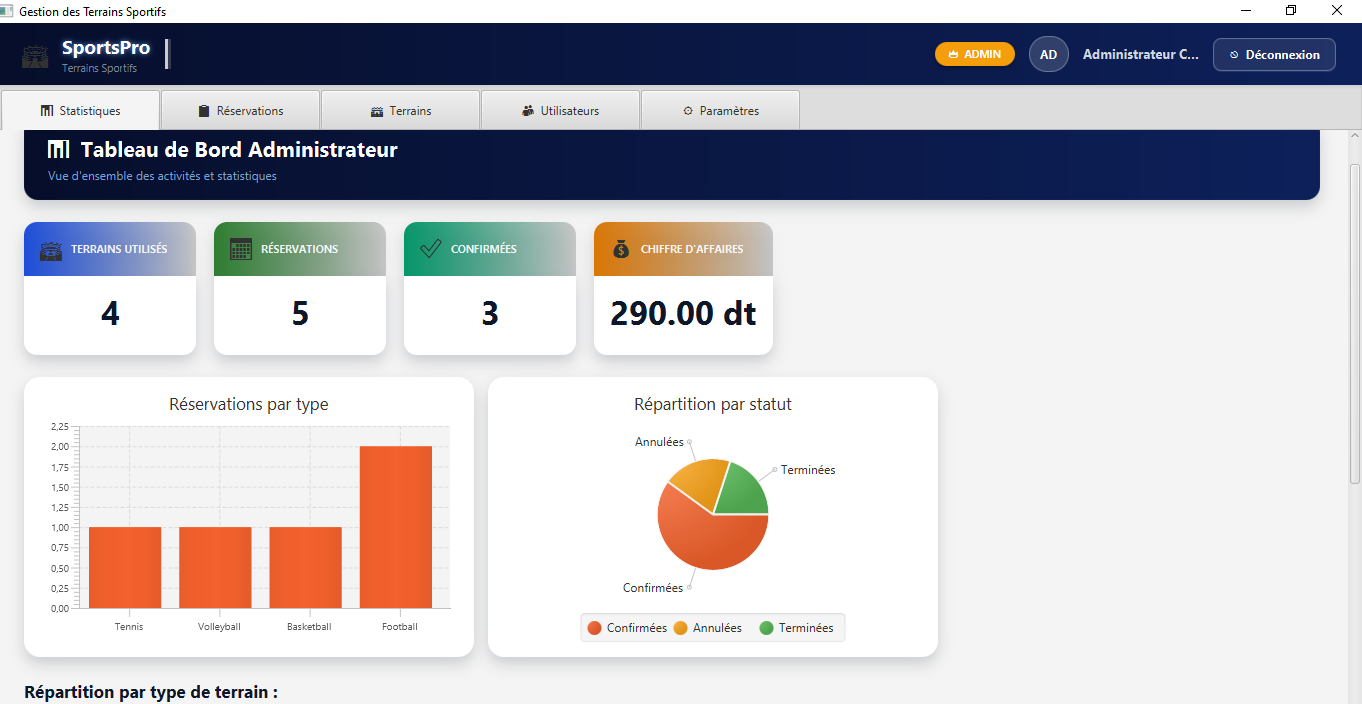
\includegraphics[width=0.95\textwidth]{rapport/images/admin_stats1.PNG}
\caption{Tableau de bord Admin — indicateurs KPI et graphiques}
\label{fig:admin_stats1}
\end{figure}

En bas de cet onglet, on trouve aussi des mini-cartes de répartition par
type de terrain et un tableau qui liste les réservations en cours
(statut CONFIRMÉE).

\begin{figure}[htbp]
\centering
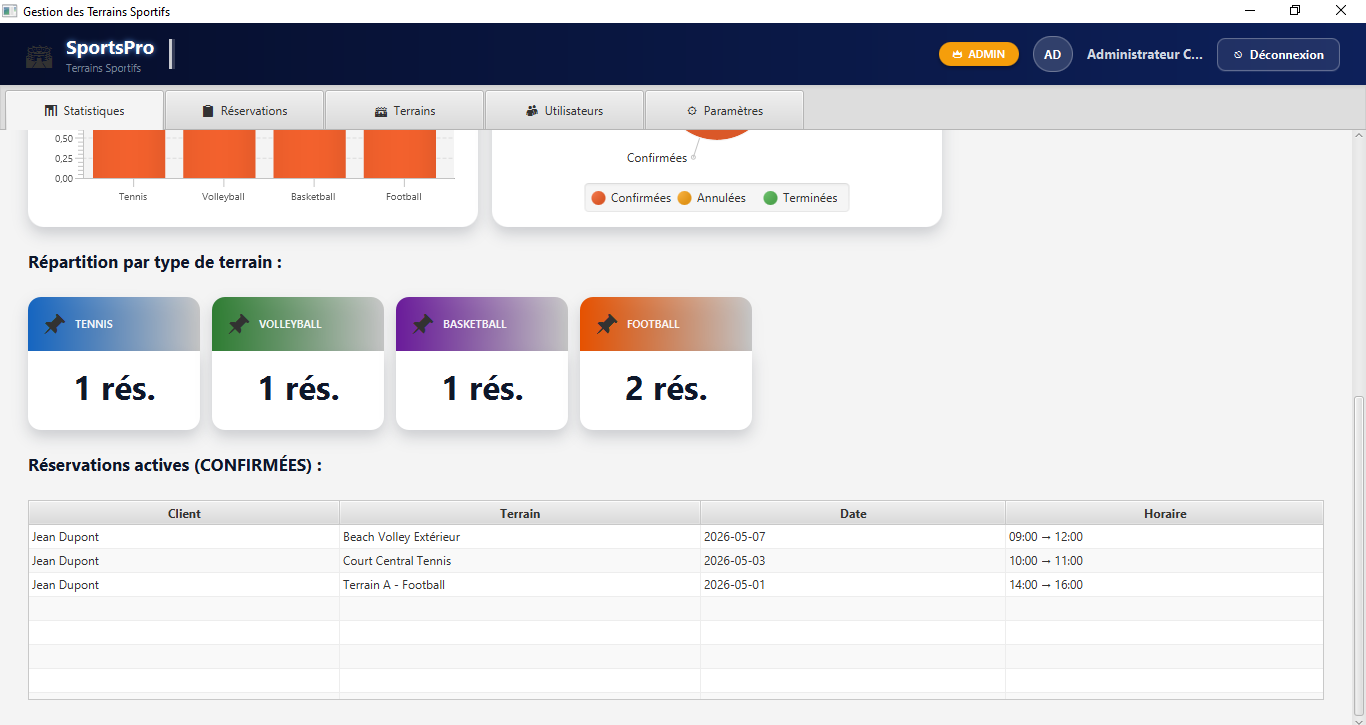
\includegraphics[width=0.95\textwidth]{rapport/images/admin_stats2.PNG}
\caption{Tableau de bord Admin — répartition par type et réservations actives}
\label{fig:admin_stats2}
\end{figure}

\subsubsection*{Onglet Réservations}

Cet onglet affiche un tableau avec toutes les réservations de tous les clients
(colonnes : ID, Client, Terrain, Date, Horaire, Montant, Statut, Action).
L'administrateur peut filtrer par statut, par période ou par mot-clé. Il peut
aussi annuler une réservation, exporter la liste en CSV ou actualiser le tableau.

\begin{figure}[htbp]
\centering
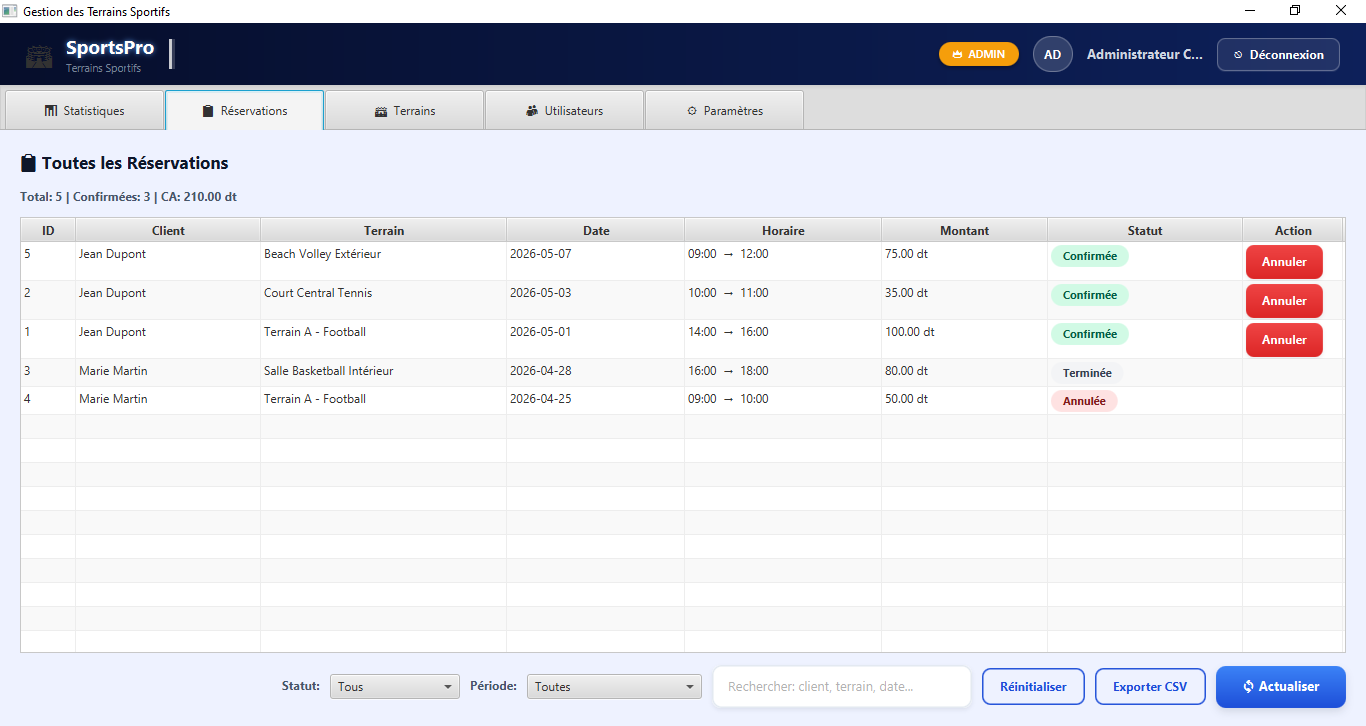
\includegraphics[width=0.95\textwidth]{rapport/images/admin_reservations.PNG}
\caption{Tableau de bord Admin — gestion de toutes les réservations}
\label{fig:admin_resa}
\end{figure}

\subsubsection*{Onglet Terrains}

Cet onglet liste tous les terrains avec leurs informations (ID, Nom, Type,
Prix/h, Statut avec \cmark{} ou \xmark{}, Description) et deux boutons
d'action : Désactiver/Activer et Supprimer. Un panneau en bas de la page
peut s'ouvrir pour ajouter un nouveau terrain directement depuis cet écran.

\begin{figure}[htbp]
\centering
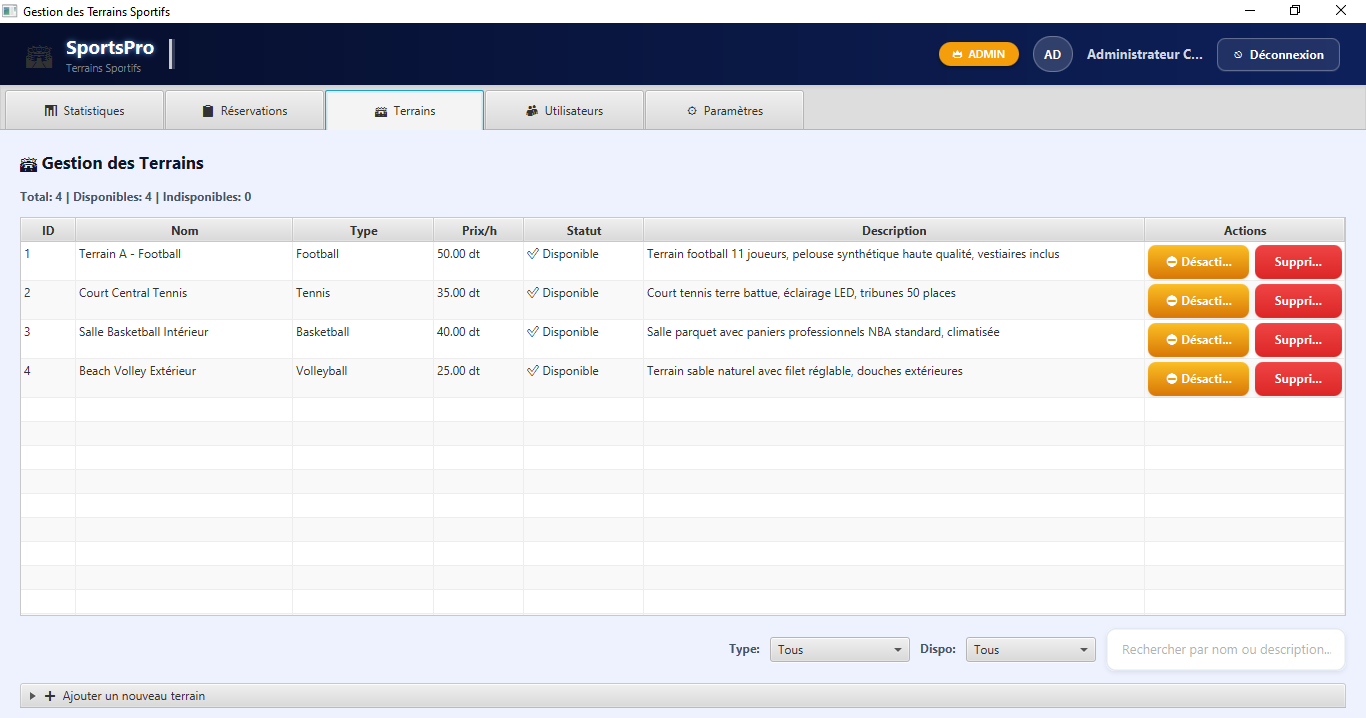
\includegraphics[width=0.95\textwidth]{rapport/images/admin_terrains.PNG}
\caption{Tableau de bord Admin — gestion des terrains sportifs}
\label{fig:admin_terrains}
\end{figure}

\subsubsection*{Onglet Utilisateurs}

Cet onglet affiche la liste de tous les comptes enregistrés (ID, Nom, Email,
Rôle, Date d'inscription). L'administrateur peut filtrer par rôle et rechercher
par nom. Le bouton Supprimer ne s'affiche que pour les comptes de type Client ;
les comptes Admin ne peuvent pas être supprimés.

\begin{figure}[htbp]
\centering
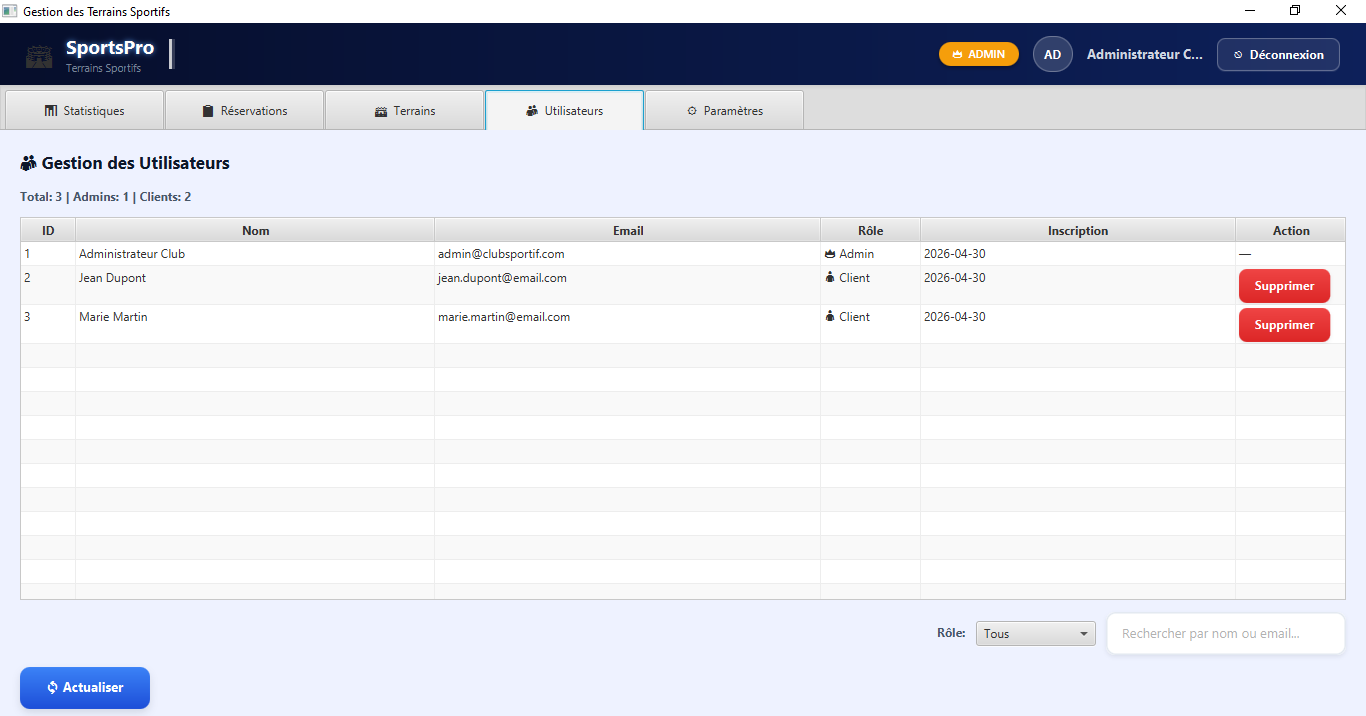
\includegraphics[width=0.95\textwidth]{rapport/images/admin_utilisateurs.PNG}
\caption{Tableau de bord Admin — gestion des comptes utilisateurs}
\label{fig:admin_users}
\end{figure}

\subsubsection*{Onglet Paramètres}

Cet onglet est divisé en deux sections. La section \textbf{Préférences} permet
de choisir le thème de l'interface (Ocean Pro, Emerald Field, Sunset Arena),
de configurer la fréquence de rafraîchissement automatique (15, 30, 60 ou
120 secondes), d'activer ou désactiver les notifications et le mode compact.
La section \textbf{Sécurité} permet de changer le mot de passe en entrant
d'abord l'ancien pour confirmer l'identité.

\begin{figure}[htbp]
\centering
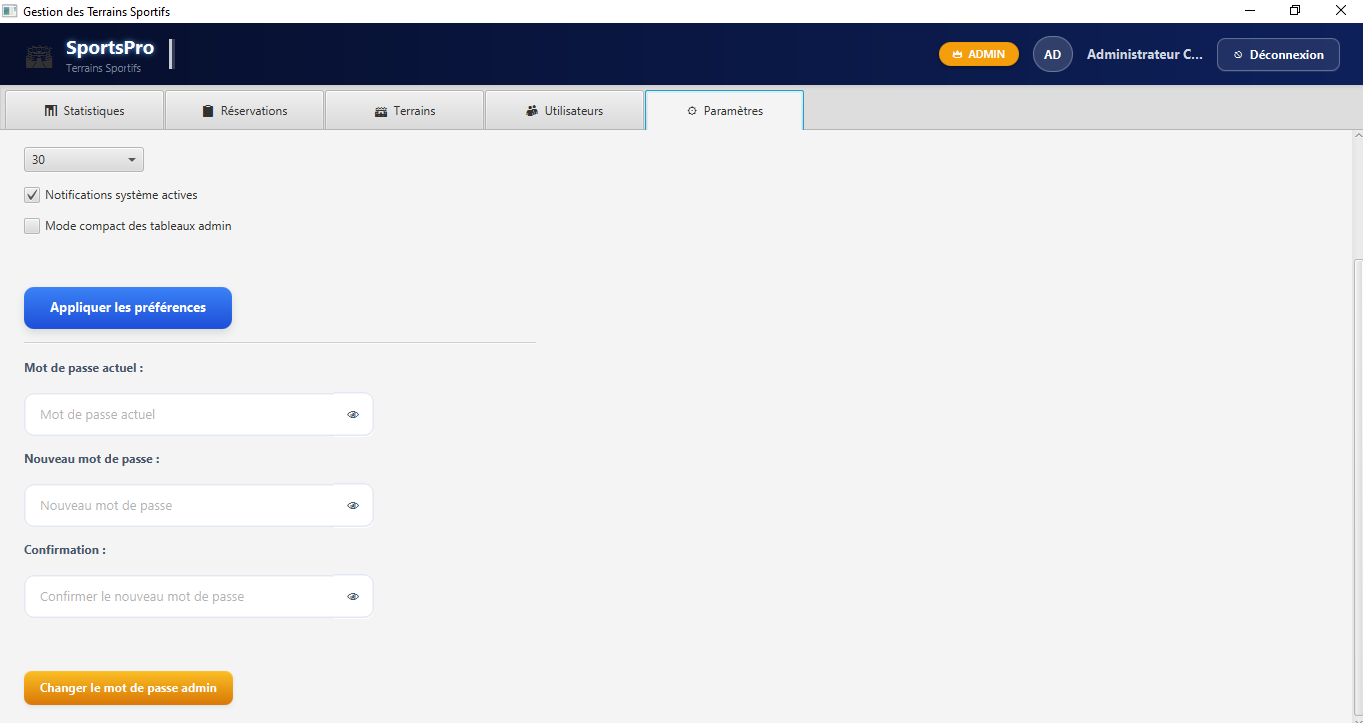
\includegraphics[width=0.78\textwidth]{rapport/images/admin_parametre.PNG}
\caption{Tableau de bord Admin — onglet Paramètres}
\label{fig:admin_params}
\end{figure}

\subsection{Tableau de bord Client}

L'interface client est aussi organisée en \textbf{cinq onglets}. La barre de
navigation affiche le nom du client, son badge CLIENT et le bouton de déconnexion.

\subsubsection*{Onglet Mes Réservations}

En haut de l'onglet, quatre statistiques personnelles s'affichent : le nombre
total de réservations, les réservations à venir, les réservations confirmées
et la dépense totale. En dessous, un tableau liste toutes les réservations du
client avec leurs détails et un bouton d'annulation pour les réservations
futures confirmées. Le client peut filtrer par statut ou par période, et
exporter la liste en CSV.

\begin{figure}[htbp]
\centering
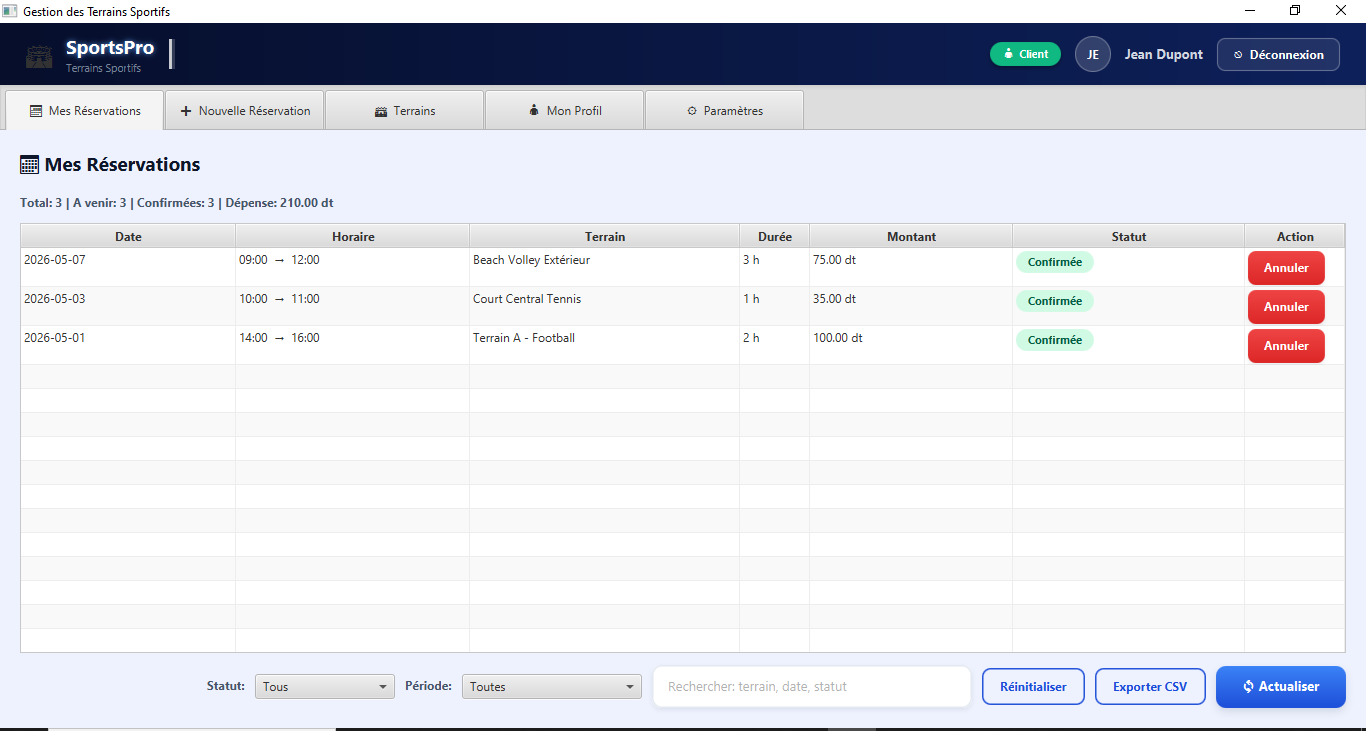
\includegraphics[width=0.95\textwidth]{rapport/images/client_historique.PNG}
\caption{Tableau de bord Client — historique des réservations}
\label{fig:client_histo}
\end{figure}

\subsubsection*{Onglet Nouvelle Réservation}

Ce formulaire guide le client pour faire une réservation : il choisit
d'abord un terrain dans la liste des terrains disponibles, puis une date,
une heure de début (entre 08h00 et 22h00) et une durée (1 à 4 heures).
Le montant estimé s'affiche en temps réel et un indicateur signale
immédiatement si le créneau est déjà pris.

\begin{figure}[htbp]
\centering
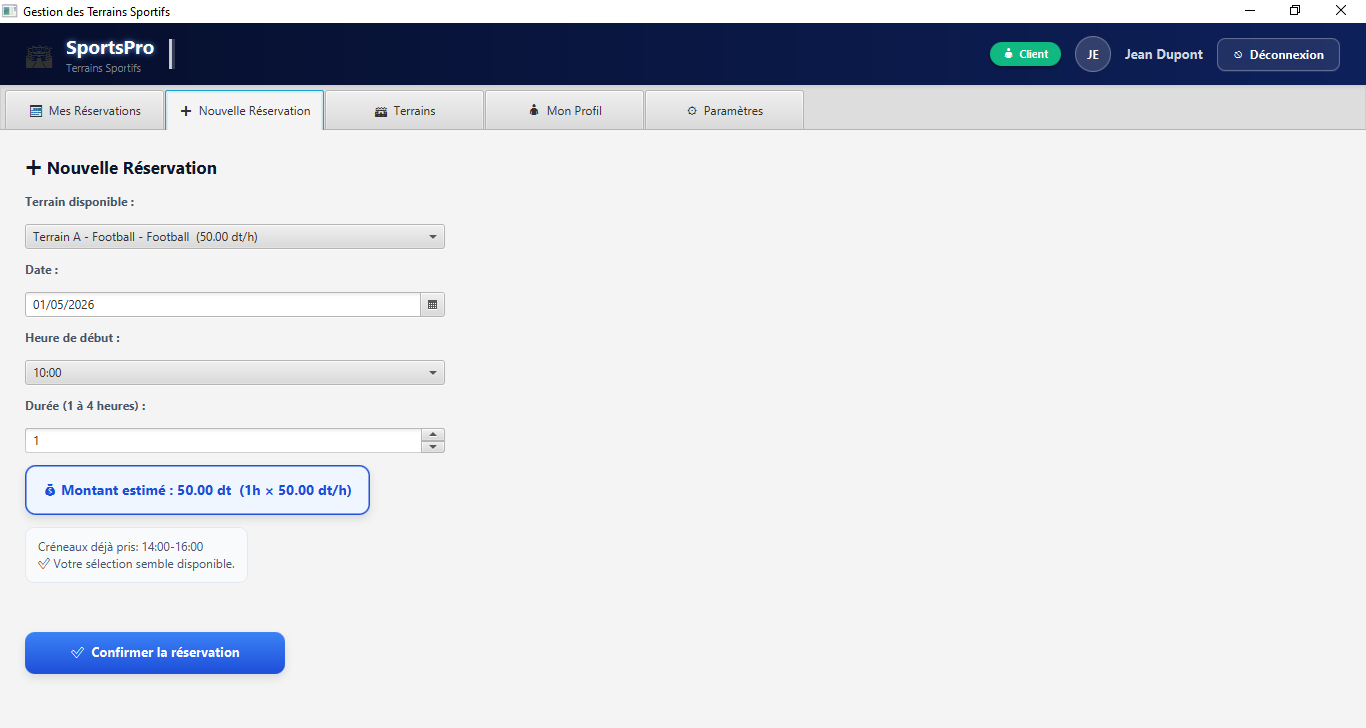
\includegraphics[width=0.85\textwidth]{rapport/images/client_reservation.PNG}
\caption{Tableau de bord Client — formulaire de nouvelle réservation}
\label{fig:client_resa}
\end{figure}

\subsubsection*{Onglets Terrains, Mon Profil et Paramètres}

\begin{itemize}
  \item \textbf{Terrains} : un tableau qui montre tous les terrains avec
        leurs caractéristiques (Nom, Type, Prix/h, Disponibilité, Description)
        pour que le client puisse comparer avant de réserver.
  \item \textbf{Mon Profil} : affiche l'e-mail et la date d'inscription
        du client, avec un formulaire pour modifier son nom, son e-mail ou
        son mot de passe.
  \item \textbf{Paramètres} : les mêmes options que pour l'administrateur
        (thème, rafraîchissement, notifications, mode compact, mot de passe).
\end{itemize}

\begin{figure}[htbp]
\centering
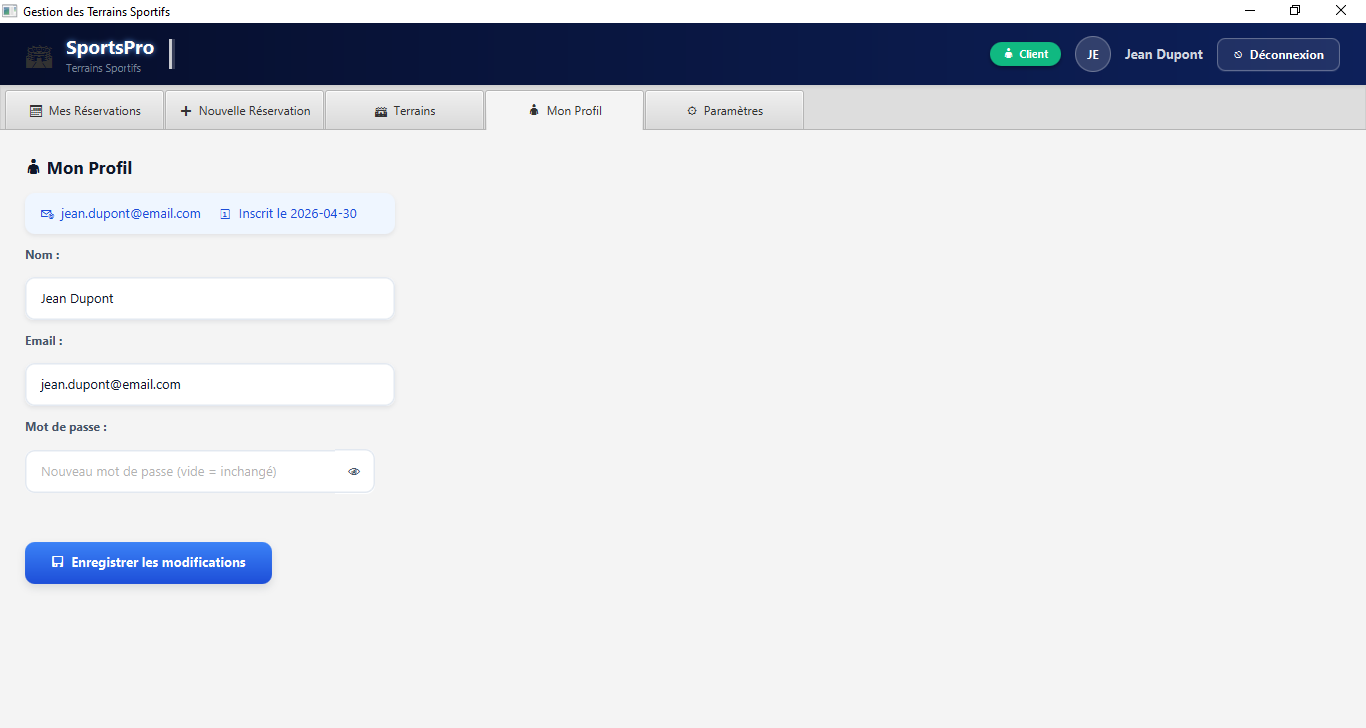
\includegraphics[width=0.78\textwidth]{rapport/images/client_profil.PNG}
\caption{Tableau de bord Client — onglet Mon Profil}
\label{fig:client_profil}
\end{figure}

% ============================================================
\chapter{Base de données}
% ============================================================

\section{Modèle Conceptuel de Données (MCD)}

Notre base de données contient trois entités principales : \textbf{UTILISATEUR},
\textbf{TERRAIN} et \textbf{RESERVATION}. La réservation est l'entité centrale
car elle fait le lien entre un utilisateur et un terrain pour un créneau
horaire précis.

Les règles de cardinalité sont les suivantes : un utilisateur peut avoir
plusieurs réservations (1-N), et un terrain peut être concerné par plusieurs
réservations (0-N).

\begin{figure}[htbp]
\centering
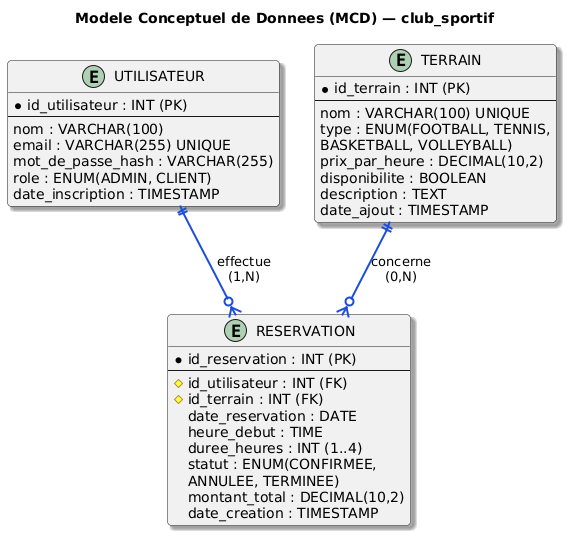
\includegraphics[width=0.95\textwidth]{rapport/images/04_mcd.png}
\caption{Modèle Conceptuel de Données — base \texttt{club\_sportif}}
\label{fig:mcd}
\end{figure}

\section{Présentation de la base de données}

La base de données \texttt{club\_sportif} est créée sous MySQL 8.0. Elle
contient \textbf{3 tables} avec des contraintes d'intégrité, des index
pour améliorer les performances et 2 vues SQL.

\subsection{Table \texttt{utilisateur}}

\begin{center}
\begin{tabular}{>{\ttfamily\small}l >{\ttfamily\small}l >{\small}l >{\small}l}
\toprule
\normalfont Colonne & \normalfont Type & Contrainte & Description \\
\midrule
id\_utilisateur      & INT            & PK, AUTO\_INCREMENT & Identifiant unique \\
nom                  & VARCHAR(100)   & NOT NULL, $\geq$2 car. & Nom complet \\
email                & VARCHAR(255)   & UNIQUE, NOT NULL   & Adresse e-mail \\
mot\_de\_passe\_hash & VARCHAR(255)   & NOT NULL           & Mot de passe haché (BCrypt) \\
role                 & ENUM           & NOT NULL           & ADMIN ou CLIENT \\
date\_inscription    & TIMESTAMP      & DEFAULT NOW()      & Date de création du compte \\
\bottomrule
\end{tabular}
\end{center}

\subsection{Table \texttt{terrain}}

\begin{center}
\begin{tabular}{>{\ttfamily\small}l >{\ttfamily\small}l >{\small}l >{\small}l}
\toprule
\normalfont Colonne & \normalfont Type & Contrainte & Description \\
\midrule
id\_terrain      & INT             & PK, AUTO\_INCREMENT & Identifiant unique \\
nom              & VARCHAR(100)    & UNIQUE, NOT NULL    & Nom du terrain \\
type             & ENUM            & NOT NULL            & Football/Tennis/Basket/Volley \\
prix\_par\_heure & DECIMAL(10,2)   & $>$ 0               & Prix par heure (en dinars) \\
disponibilite    & BOOLEAN         & DEFAULT TRUE        & Disponible (true) ou non (false) \\
description      & TEXT            & Optionnel           & Description du terrain \\
date\_ajout      & TIMESTAMP       & DEFAULT NOW()       & Date d'ajout \\
\bottomrule
\end{tabular}
\end{center}

\subsection{Table \texttt{reservation}}

\begin{center}
\begin{tabular}{>{\ttfamily\small}l >{\ttfamily\small}l >{\small}l >{\small}l}
\toprule
\normalfont Colonne & \normalfont Type & Contrainte & Description \\
\midrule
id\_reservation   & INT            & PK, AUTO\_INCREMENT & Identifiant unique \\
id\_utilisateur   & INT            & FK $\to$ utilisateur & Référence au client \\
id\_terrain       & INT            & FK $\to$ terrain    & Référence au terrain \\
date\_reservation & DATE           & NOT NULL            & Date du créneau \\
heure\_debut      & TIME           & 08:00–22:00         & Heure de début \\
duree\_heures     & INT            & 1 à 4               & Durée en heures \\
statut            & ENUM           & NOT NULL            & CONFIRMEE/ANNULEE/TERMINEE \\
montant\_total    & DECIMAL(10,2)  & $>$ 0               & Montant calculé \\
date\_creation    & TIMESTAMP      & DEFAULT NOW()       & Date d'enregistrement \\
\bottomrule
\end{tabular}
\end{center}

\subsection{Capture de la structure de la base}

La base de données est créée en exécutant le fichier \texttt{database.sql}
fourni avec le projet. Ce script crée les trois tables, les index, les deux
vues SQL (\texttt{v\_reservations\_actives} et \texttt{v\_stats\_terrain})
et insère des données de test (un compte admin, un compte client et trois
terrains).

Pour initialiser la base, on exécute la commande suivante dans le terminal :
\begin{center}
\texttt{mysql -u root -p < database.sql}
\end{center}

La capture ci-dessous, prise depuis phpMyAdmin, montre la structure de
la base \texttt{club\_sportif} avec ses trois tables.

\begin{figure}[htbp]
\centering
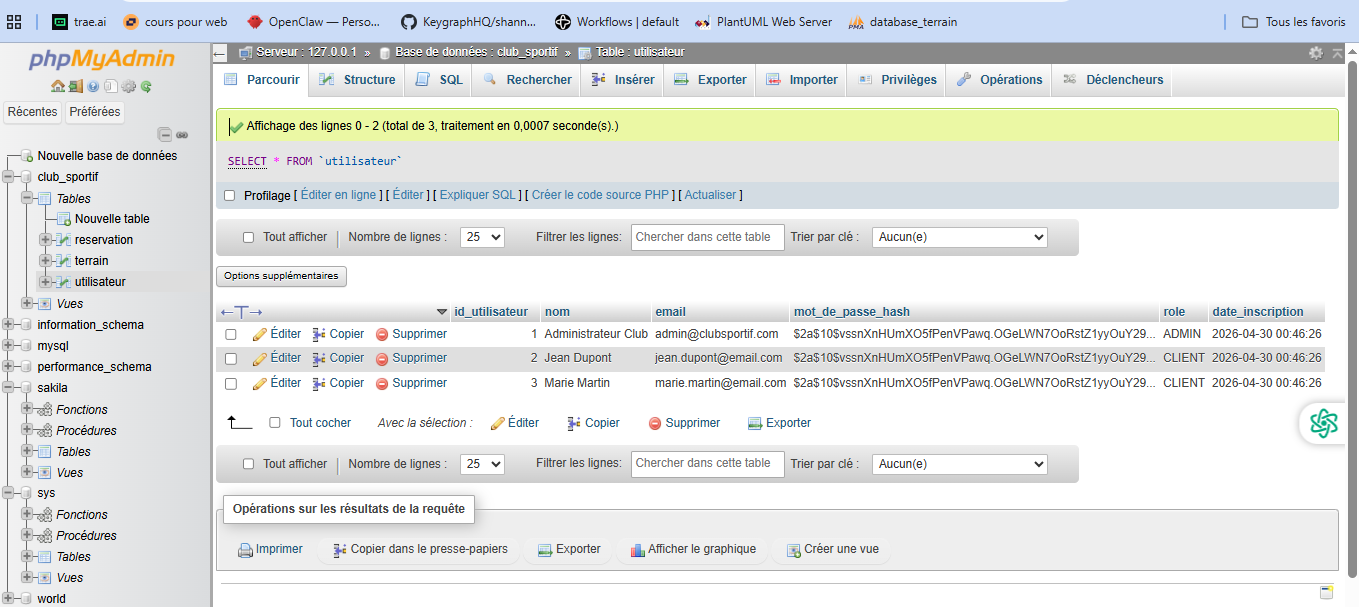
\includegraphics[width=0.95\textwidth]{rapport/images/structure_database.PNG}
\caption{Structure de la base \texttt{club\_sportif} — phpMyAdmin}
\label{fig:db}
\end{figure}

% ============================================================
\chapter{Difficultés rencontrées}
% ============================================================

\section{Problèmes techniques rencontrés}

Pendant le développement du projet, nous avons rencontré plusieurs problèmes
techniques que nous avons dû analyser et résoudre.

\begin{enumerate}

  \item \textbf{Détection des conflits de créneaux horaires}

  Au début, nous n'étions pas sûrs de la bonne condition pour détecter
  si deux créneaux se chevauchent. Après réflexion, nous avons trouvé
  la règle suivante : deux créneaux $[A,\,B]$ et $[C,\,D]$ se chevauchent
  si $A < D$ \textbf{et} $C < B$. Nous avons mis cette logique dans une
  classe séparée (\texttt{OverlapUtils}) et nous l'avons testée avec des
  tests unitaires JUnit 5 pour vérifier tous les cas possibles.

  \item \textbf{Problème de lancement du JAR avec JavaFX}

  Quand on essayait de lancer l'application avec la commande
  \texttt{java -jar}, on obtenait une erreur. Le problème vient du fait
  que depuis Java 9, une classe qui hérite de \texttt{Application} (JavaFX)
  ne peut pas être le point d'entrée direct d'un JAR. Pour résoudre ce
  problème, nous avons créé une classe \texttt{Launcher} simple qui ne
  hérite d'aucune classe JavaFX et qui appelle simplement
  \texttt{MainApp.main(args)}.

  \item \textbf{Configuration de la connexion MySQL}

  Les paramètres de connexion à MySQL (adresse, port, mot de passe) sont
  différents sur chaque machine. Au lieu de modifier le code à chaque fois,
  nous avons centralisé tous ces paramètres dans une seule classe
  \texttt{AppConfig.java}. Ainsi, pour adapter l'application à une nouvelle
  machine, il suffit de modifier ce seul fichier.

  \item \textbf{Construction du fichier JAR avec toutes les dépendances}

  Au départ, le fichier JAR généré par Maven ne contenait pas les bibliothèques
  JavaFX et jBCrypt. L'application ne pouvait donc pas se lancer sur une autre
  machine. Nous avons résolu ce problème en configurant le plugin
  \texttt{maven-assembly-plugin} dans le fichier \texttt{pom.xml} pour créer
  un JAR complet qui embarque toutes les dépendances.

\end{enumerate}

\section{Problèmes organisationnels rencontrés}

\begin{enumerate}

  \item \textbf{Répartition du travail}

  Au début du projet, nous avons eu du mal à décider qui fait quoi pour
  éviter que deux personnes travaillent sur le même fichier en même temps.
  Nous avons finalement décidé que chaque membre prend en charge une
  fonctionnalité complète de la base de données jusqu'à l'interface : une
  personne s'occupe de tout ce qui concerne les terrains, l'autre s'occupe
  des réservations.

  \item \textbf{Incompatibilité de nos environnements}

  Nos deux machines n'avaient pas la même configuration MySQL : l'une
  n'avait pas de mot de passe root et l'autre en avait un. Chacun avait
  aussi une version différente de MySQL. La solution était de mettre tous
  les paramètres de connexion dans le fichier \texttt{AppConfig.java}
  et de mettre à jour ce fichier selon la machine utilisée.

  \item \textbf{Sous-estimation du temps pour les livrables}

  Nous avons mis plus de temps que prévu pour réaliser les diagrammes UML
  et rédiger le rapport. Si nous devions recommencer, nous planifierions
  ces tâches dès le début du projet et non pas à la fin.

\end{enumerate}

% ============================================================
\chapter{Conclusion}
% ============================================================

\section*{Ce que nous avons réalisé}

Ce mini projet nous a donné l'occasion de développer une application Java
complète et fonctionnelle, de la conception jusqu'au déploiement. Nous sommes
partis d'une analyse des besoins, nous avons conçu les diagrammes UML, nous
avons développé le code en suivant une architecture organisée, et nous avons
livré une application exécutable avec une interface graphique moderne.

L'application \textbf{SportsPro} répond à tous les objectifs fixés au départ :
les clients peuvent réserver des terrains facilement, et les administrateurs
peuvent gérer le système depuis un tableau de bord complet. Le tout avec
une sécurité correcte des données et une interface agréable à utiliser.

\section*{Ce que nous avons appris}

Ce projet nous a permis d'appliquer en pratique plusieurs notions importantes :

\begin{itemize}
  \item Organiser une application Java avec une \textbf{architecture en couches}
        (MVC + DAO + Service) pour que le code soit propre et facile à modifier.
  \item Connecter une application Java à une base de données \textbf{MySQL via
        JDBC} et écrire des requêtes SQL avec \texttt{PreparedStatement} pour
        éviter les problèmes de sécurité.
  \item Créer des interfaces graphiques \textbf{JavaFX} avec des tableaux,
        des graphiques, des formulaires et plusieurs thèmes visuels.
  \item Sécuriser les mots de passe avec l'algorithme \textbf{BCrypt} et
        valider les données saisies par l'utilisateur.
  \item Écrire des \textbf{tests unitaires} avec JUnit 5 et simuler les
        dépendances avec Mockito pour tester la couche Service.
  \item Utiliser \textbf{Maven} pour gérer les dépendances et créer un
        fichier JAR exécutable autonome.
\end{itemize}

\section*{Améliorations possibles}

Si nous avions plus de temps, nous aimerions ajouter les fonctionnalités
suivantes à l'application :
\begin{itemize}
  \item L'envoi automatique d'un e-mail de confirmation après chaque
        réservation.
  \item Un système de paiement en ligne intégré directement dans
        l'application.
  \item Une version web de l'application (avec Spring Boot et un framework
        JavaScript) pour qu'elle soit accessible depuis n'importe quel
        navigateur sans installation.
\end{itemize}

\end{document}
